\section{Magnetic field}

\begin{Exercise}[difficulty=1]
Find direction and value of magnetic field H produced by current I in the point P. 
\begin{center}
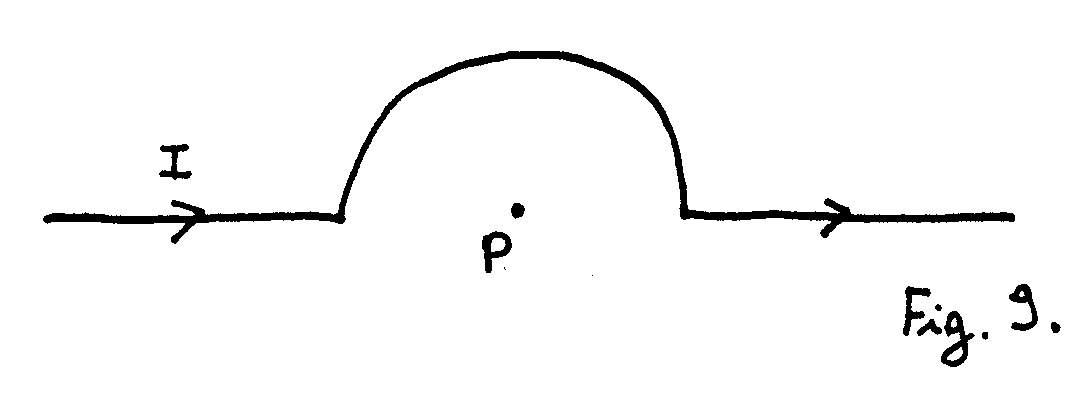
\includegraphics[width=0.4\textwidth]{img/fig_m1.png} 
\end{center}
\end{Exercise}

\begin{Exercise}[difficulty=3]
Using Ampere's Circular Law describe distribution of magnetic field vector inside, and outside coaxial cable.
\begin{center}
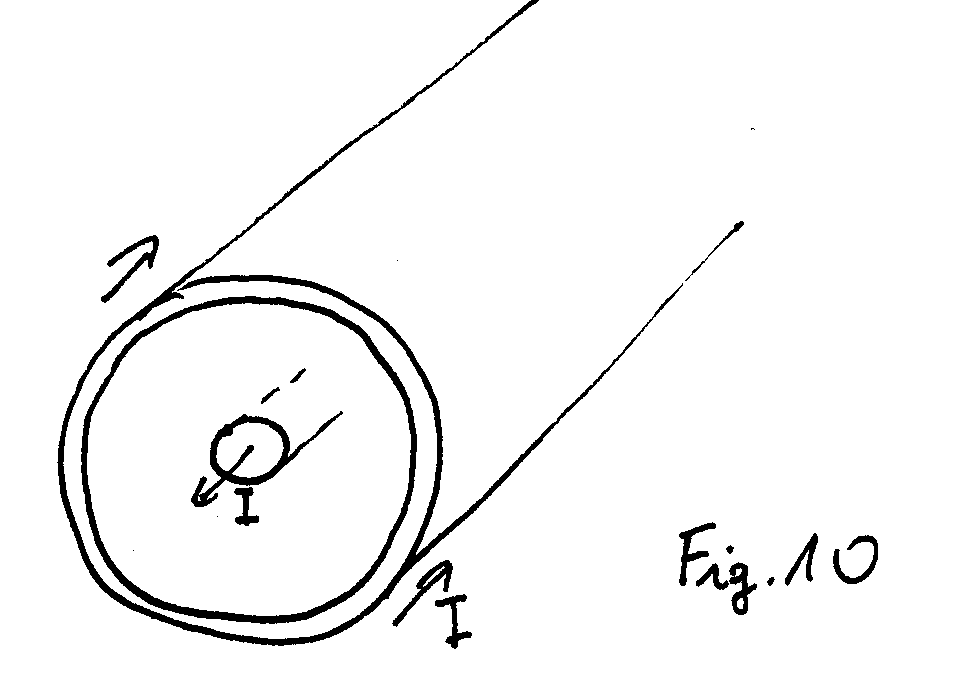
\includegraphics[width=0.4\textwidth]{img/fig_m2.png} 
\end{center}
\end{Exercise}

\begin{Exercise}[difficulty=2]
Two long, parallel cables with the same values but opposite directions of DC current are producing magnetic field around them. Find H distribution on the plane defined by two cables. 
\begin{center}
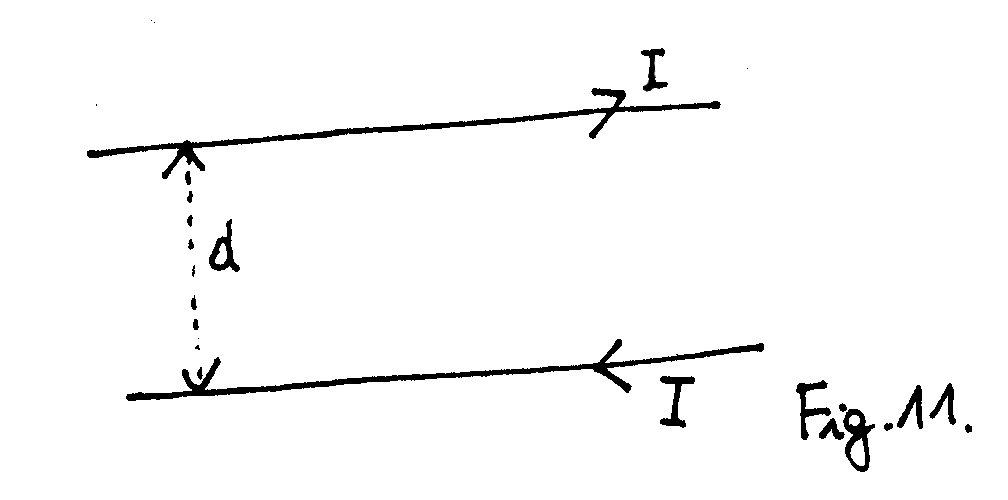
\includegraphics[width=0.4\textwidth]{img/fig_m3.png} 
\end{center}
\end{Exercise}

\begin{Exercise}[difficulty=3]
Square shape conducting frame (size $a$ by $a$) is placed in the distance of $a$ from the straight cable. Magnetic coupling between these circuits can be observed. Find mutual inductance. 
\begin{center}
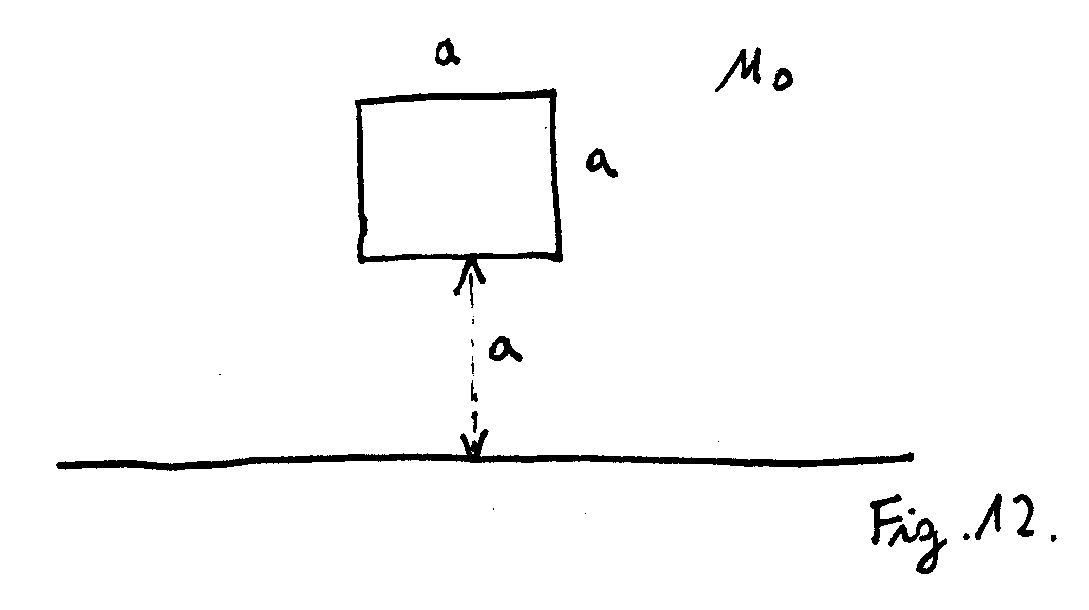
\includegraphics[width=0.4\textwidth]{img/fig_m4.png} 
\end{center}
\end{Exercise}

\begin{Exercise}[difficulty=3]
What is the magnetic flux in the toroidal core (cross-section of the coil is square ($h$ by $h$), internal radius is $R$). There are $n$ turns around the core, and value of the flowing current is $I$.
\begin{center}
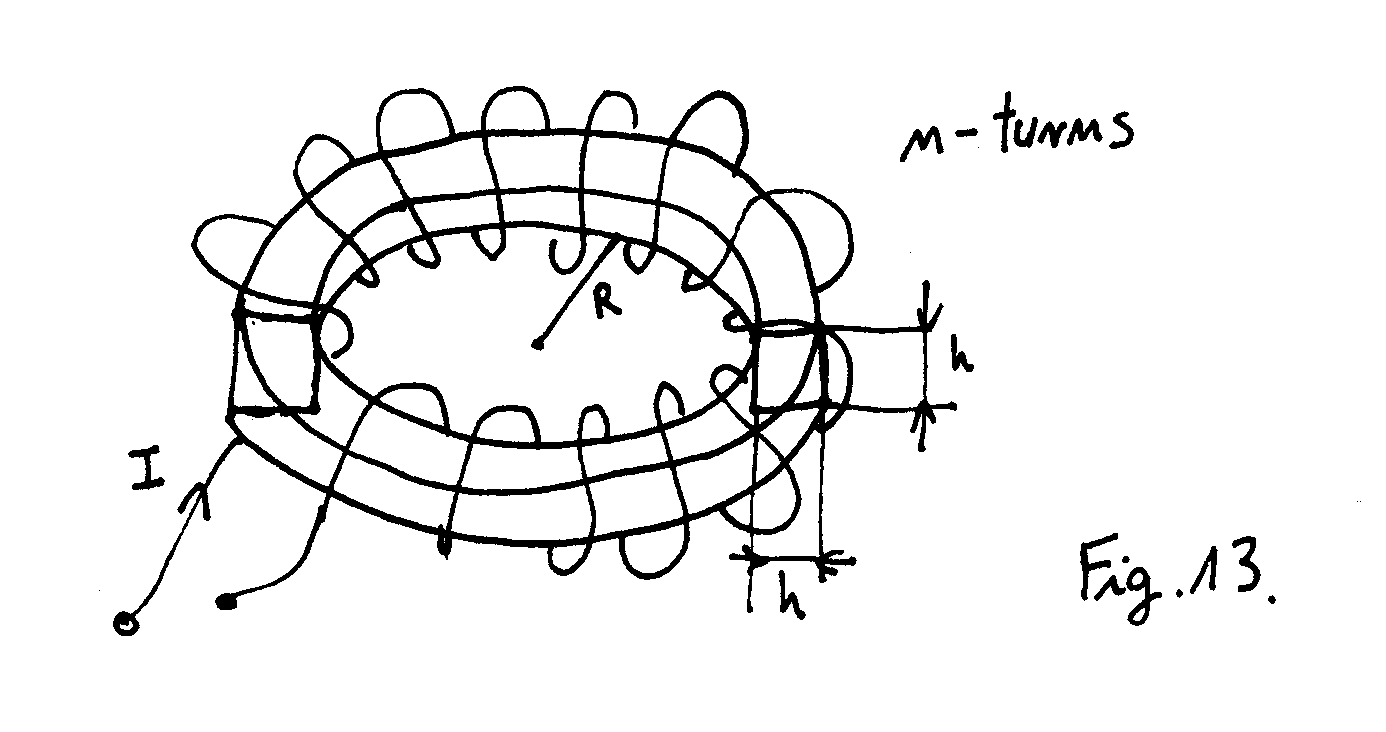
\includegraphics[width=0.4\textwidth]{img/fig_m5.png} 
\end{center}
\end{Exercise}

\begin{Exercise}[difficulty=2]
Find value and direction of magnetic field vector in the point P. As shown on the figure below, point P is in the middle of set of four parallel conducting lines, where in three of them current is flowing in the same direction, hence in one in opposite direction.
\begin{center}
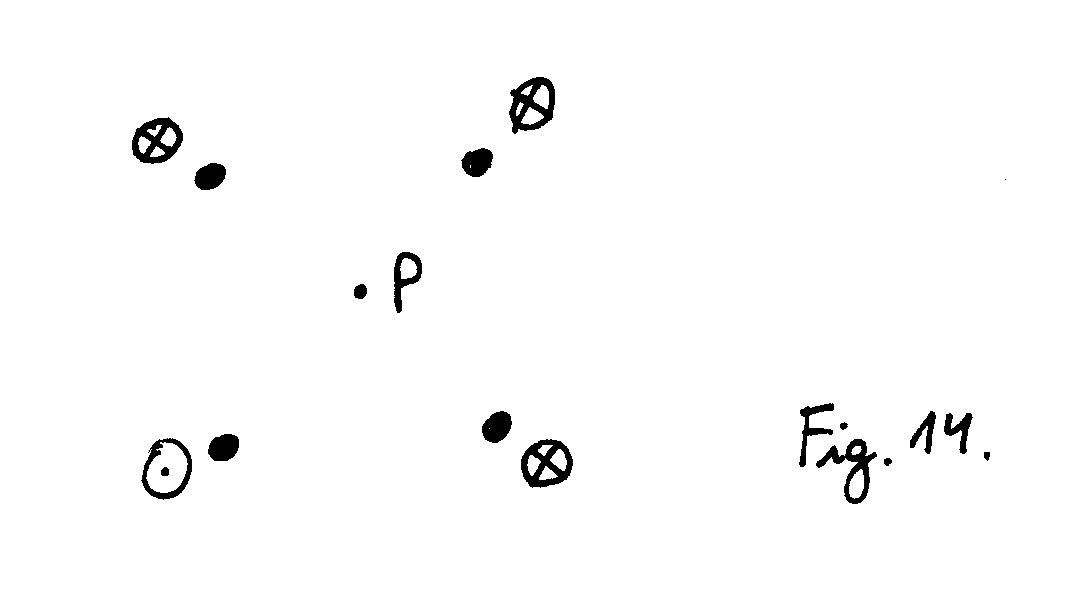
\includegraphics[width=0.4\textwidth]{img/fig_m6.png} 
\end{center}
\end{Exercise}



